%Este trabalho está licenciado sob a Licença Creative Commons Atribuição-CompartilhaIgual 3.0 Não Adaptada. Para ver uma cópia desta licença, visite https://creativecommons.org/licenses/by-sa/3.0/ ou envie uma carta para Creative Commons, PO Box 1866, Mountain View, CA 94042, USA.

\usepackage[a4paper,headheight=15.4pt]{geometry}

%%%%%%%%%%%%%%%%%%%%%%%%%%%%%%%%%%%%%%%%%
% ATENÇÃO
%
% POR SEGURANÇA, NÃO EDITE ESTE ARQUIVO.
%
%%%%%%%%%%%%%%%%%%%%%%%%%%%%%%%%%%%%%%%%%


%%%%%%%%%%%%%%%%%%%%%%%%%%%%%%%%%
%  ambientes 
%%%%%%%%%%%%%%%%%%%%%%%%%%%%%%%%%
  \theoremstyle{plain}          %   bold title, italic body
  \newtheorem{teo}{Teorema}[section]
  \newtheorem{lem}{Lema}[section]
  \newtheorem{prop}{Proposição}[section]
  \newtheorem{corol}{Corolário}[section]
  \newtheorem{defn}{Definição}[section]
  \theoremstyle{remark}           % italic title, romman body
  \theoremstyle{definition}       % italic title, romman body
  \newtheorem{obs}{Observação}[section]
  \newtheorem{ex}{Exemplo}[section]

%%%% titlepage figure %%%%
\usepackage{eso-pic}
\newcommand\BackgroundPic{%
\put(0,0){%
\parbox[b][\paperheight]{\paperwidth}{%
\vfill
\centering
\includegraphics[width=\paperwidth,height=\paperheight,%
keepaspectratio]{./rosto/capa.eps}%
\vfill
}}}

%%%%%%%%%%%%%%%%%%%%%%%%%%%%%%%
%%%% Exercises and Answers %%%%
%\usepackage[lastexercise]{exercise}
\usepackage[answerdelayed,lastexercise]{exercise}
\usepackage{chngcntr}
\counterwithin{Exercise}{section}
\counterwithin{Answer}{section}
\renewcommand{\ExerciseHeaderTitle}{({\it \ExerciseTitle})}
\renewcommand{\ExerciseName}{E}
\renewcommand{\ExerciseHeader}{{\textbf{\large\ExerciseName~\ExerciseHeaderNB\ExerciseHeaderTitle\ExerciseHeaderOrigin}}}
\renewcommand{\ExerciseHeader}{\textbf{\ExerciseName\ \ExerciseHeaderNB.}\,}

% change font for answers header
\renewcommand{\AnswerHeader}{\tiny\textbf{\ExerciseName\ \ExerciseHeaderNB.}\smallskip}
% change font for answers list header
\renewcommand{\AnswerListHeader}{{\tiny\textbf{\AnswerListName\
(\ExerciseListName\ \ExerciseHeaderNB)\ ---\ }}}
%%%%%%%%%%%%%%%%%%%%%%%%%%%%%%


\newenvironment{exer}
{\begin{Exercise}}
{\end{Exercise}}

\newenvironment{resp}
{\begin{Answer}\begin{tiny}}
{\end{tiny}\end{Answer}}

\newenvironment{sol}
{\let\oldqedsymbol=\qedsymbol
  \renewcommand{\qedsymbol}{$\Diamond$}
  \begin{proof}[\bfseries\upshape Solução]}
  {\end{proof}
  \renewcommand{\qedsymbol}{\oldqedsymbol}}

%%%%%%%%%%%%%%%%%%%%%%%%%%%%%%
% Exercícios Resolvidos
%%%%%%%%%%%%%%%%%%%%%%%%%%%%%%
\newtheorem{exeresol}{ER}[section]
\newenvironment{resol}
{\let\oldqedsymbol=\qedsymbol
  \renewcommand{\qedsymbol}{$\Diamond$}
  \begin{proof}[\bfseries\upshape Solução]}
  {\end{proof}
  \renewcommand{\qedsymbol}{\oldqedsymbol}}
%%%%%%%%%%%%%%%%%%%%%%%%%%%%%%
